\documentclass[font =22]{report}
\usepackage{amsmath}
\title{Differential Equations Notes}
\author{Tyler Lukasiewicz}
\date{\copyright\;2014\\All Rights Reserved}
\usepackage{amsmath}
\usepackage{amsfonts}
\usepackage{float}
\usepackage{graphicx}
\usepackage{algorithmicx}
\usepackage{algpseudocode} 
\usepackage{caption}
\usepackage{subcaption}
\usepackage{graphicx}
\usepackage{textcomp}
\setlength{\textheight}{8.5in}
\setlength{\topmargin}{0.5in}
\setlength{\headheight}{0.in}
\setlength{\headsep}{0in}
\setlength{\oddsidemargin}{0in}
\setlength{\textwidth}{6.5in}

\begin{document}

\maketitle
\tableofcontents

\chapter{First Order Differential Equations}
\section{A Few Words On Differential Equations}
\paragraph{}
Wikipedia describes a differential equation as ``a mathematical equation that relates some function of one or more variables with its derivatives".
Khan academy gives the definition of ``an equation that involves some unknown function and it's derivatives". I prefer the latter definition, as it emphasizes the operative word `unknown'. Up to this point, whenever we have `solved' an equation, we have found some number  or set of numbers that satisfy the equation. For example the equation $x^2+4x+3  = 0$, is true when $x=-1$ and $x=-3$. $x$ in this case, was the unknown. When presented with a differential equation, we are not looking for a number or a set of numbers. We are trying to find a function that satisfies the criteria that we are given. 

\paragraph{}
In order to get a better grasp of exactly what we are doing, let's work backwards from the answer and create a differential equation.
\\
We'll will start with a simple equation: $f(x) = x^3 + 3x^2 +x$.
We know from calc 1 that \[f'(x) = 3x^2 + 6x +1 \]
and \[ f''(x) = 6x+6. \]
Let's create a differential equation.

\begin{align*}
f'(x) +f''(x) &= (3x^2 + 6x +1) +  (6x+6) 
\\&= 3x^2 +12x+7 
\end{align*}
\paragraph{}
And there we have it! our very own differential equation. Written slightly differently :
$y'+y'' = 3x^2 +12x+7$.\\
The solution $y = x^3 + 3x^2 +x$ may be obvious to us, but if we were to give someone else the differential equation $y'+y'' = 3x^2 +12x+7$, they may disagree.

\paragraph{}
 A  differential equation is usually used to represent some real life scenario, where the parameter $t$ represents time.  Let's take a look at a simple example: 
\[
\frac{dx}{dt} = x(t).
\]
We don't immediately know what the function $x(t)$ is. However, we do know how $x(t)$ changes with respect to time. Imagine that $x(t)$ is a position function. What this differential equation is telling us is that the velocity $\dfrac{dx}{dt}$ is equal to the position. So as the object moves forward, it also accelerates.
In this case, $x(t)$ is the exponential function. However, what may not be immediately intuitive is that the majority of differential equations are not solvable. That is, there is no  explicit solution that always satisfies the given criteria that can be solved for with conventional mathematics. However, there are some special cases in which we can use various techniques to find an explicit solution. In this class, we will be learning these techniques and when they can be applied. 



\section{Integrating Factors }
\paragraph{}
 Consider the  equation in the form of 
\[ \frac{dy}{dt} + p(t)y = g(t)\]
where $p(t)$ and $g(t)$ are both continuous. We want to find some function $ \mu (t)$ such that 
  \[
  \frac{d}{dt}[\mu (t)y] = \mu(t)\frac{dy}{dt} + \mu(t)p(t)y = \mu(t)g(t).
  \] 
 Applying the chain rule to $\dfrac{d}{dt}[\mu (t)y]$,  we get 
\[
\frac{d}{dt}[\mu (t)y] = \mu(t) \frac{dy}{dt}  + \frac{d\mu}{dt}y.
\]
we want
 \[ 
 \mu(t) \frac{dy}{dt}  + \frac{d\mu}{dt}y = \mu(t)\frac{dy}{dt} + \mu(t)p(t)y 
 \]
 so
 \[
\frac{d\mu}{dt}y = p(t)\mu(t)y .  
\]
\[
  \frac{d\mu}{dt} = p(t)\mu(t)
 \]
 This is now a separable equation that we can easily integrate.
 \[
 \int \frac{d\mu}{\mu(t)}\ =  \int p(t)\,dt
 \]
 \[
 \ln|\mu(t)| + C = \int p(t)\,dt
 \]
 lets choose $C=0$ to obtain the simplest possible function for $\mu(t)$
 \[
 \mu(t) = \exp\int p(t) \,dt
 \]
   
\paragraph{}
In general, regarding an equation in the form of
\[
\frac{dy}{dt}+p(t)y = g(t),
\]
where both $p(t)$ and $g(t)$ are continuous, we can set $\mu (t) $ equal to 
\[
\exp \int p(t)\,dt 
\]
and multiply the equation by $\mu(t)$ so that 
\[
\frac{d}{dt}[\mu(t)y] = \frac{dy}{dt}\mu(t) + \mu(t)p(t)y = \mu(t)g(t)
\]
\[
\mu(t)y=\int \mu(t)g(t)\,dt+C
\]
and finally 
\[
y = \frac{1}{\mu(t)} \left(\int \mu(t)g(t)\,dt + C\right).
\]
So, we have proven that the solution to any differential equation in the form of 
\[
\frac{dy}{dt} + p(t)y = g(t)
\]
is
\[
y(t) = \frac{1}{\mu(t)}\left(\int \mu(t)g(t)\,dt+C\right)
\]
where 
\[
\mu(t) =\exp \int p(t)\,dt 
\]
as long as $p(t)$ and $g(t)$ are continuous.


\paragraph{}
Now, let's take this idea a bit further. We are going to attempt to find an explicit solution to any equation in the form of 
\[
\frac{dy}{dt} + p(t)y = g(t)
\]
where we are given some initial value of $t$: $t_0$, and the initial condition $y(t_0) = y_0$.
We want to set our limits of integration from some given initial value $t_0$ to some arbitrary value $t$.
so we have
\[
\mu(t) = \exp \int_{t_0}^t p(s)\,ds
\]
plugging in our given initial value $t_0$ we get
\[
\mu(t_0)=\exp \int_{t_0}^{t_0} p(s)\,ds 
\]
so
\[
\mu(t_0) = e^0
\]
\[
\mu(t_0) = 1
\]
Let's apply this same method to $y(t)$ . 
\[
y(t) = \frac{1}{\mu(t)}\left(\int_{t_0}^{t} \mu(s)g(s)\,ds+C\right)
\]
\[
y(t_0) = \frac{1}{\mu(t_0)}\left(\int_{t_0}^{t_0} \mu(s)g(s)\,ds + C \right)
\]
\[
y(t_0) = C
\]
but $y(t_0) = y_0$, so $C = y_0$
and 
\[
y = \frac{1}{\mu(t)}\left(\int_{t_0}^{t} \mu(s)g(s)\,ds + y_0 \right)
\]
So we have proven that as long as $p(t)$ and $g(t)$ are continuous on some interval of $t$ containing $t_0$, there is a function that satisfies the differential equation 
\[
\frac{dy}{dt} + p(t)y = g(t) 
\]
as well as the initial condition $y(t_0) = y_0$


\subsection*{Theorem}
\paragraph{}
This brings us to our fist theorem. If the given functions p and g are continuous on an open interval $I: \alpha<t<\beta$ containing the point $t = t_0$, then there exists a unique function $y = \phi(t)$ that satisfies the differential equation 
\[
y'+p(t)y=g(t)
\]
for each $t$ in $I$, and that also satisfies the initial condition $y(t_0) = y_0$, where $y_0$ is an arbitrary prescribed initial value.


\subsection*{Example}
\paragraph{}
Solve the initial value problem and determine the interval in which the
solution exists depends on the initial value $y_0$

\paragraph{}
1)
$y'+y^3 = 0$;      $y(0) = y_0$\\\\
For this example, we will assume that you can find the explicit solutions to this separable equation:
\[
y =  \frac{{y_0}}{\sqrt{2ty_0^2+1}}; y_0\neq 0
\]
\[
y=0; y_0 = 0
\]
So let's find the restrictions on this equation. 
\\We know that if $y_0 \neq 0$, then $2ty_0^2+1 \neq$ 0
\\and that $\dfrac{{y_0}^2}{2ty_0^2+1}$ must be $\geq 0$
so we'll set $2ty_0^2+1 = 0$ and we find that $t$ must be $> \dfrac{-1}{2y_0^2}$




\section{Exact Equations}
\subsection{Calc III Review}
\paragraph{}
Before we start on this particular method, let's do a small review of Calc III. When a function contains more than one variable i.e. $f(y,x)$, we can take what's called a partial derivative. A partial derivative of a function of several variables is its derivative with respect to one of those variables, with the others held constant (as opposed to the total derivative, in which all variables are allowed to vary). For example, if we have the function 
\[
f(x,y) = x^2+y, 
\]
than the partial with respect to x, denoted as $\dfrac{\partial f}{\partial x}$  or $f_x = 2x$. and 
$\dfrac{\partial f}{\partial y}$ or $f_y = 1$

\subsection*{The chain rule}
\paragraph{}
Let z be a differentiable function of x and y, where x and y are differentiable functions of s and t. Then
\[
\frac{d z}{d t} = \frac{\partial z}{\partial x}\frac{dx}{dt}  + \frac{\partial z}{\partial y} \frac{dy}{dt}
\]
and
\[ 
\frac{d z}{d s} = \frac{\partial z}{\partial x}\frac{dx}{ds}  + \frac{\partial z}{\partial y} \frac{dy}{ds}
\]
Note: There is a proof for this, but It's not very important for this class. 
\\\\ 
so if we have some function $\psi(x,y)$ where $y=\phi(x)$,
than 
\[
\frac{d}{dx}[\psi(x,\phi(x))]= \frac{\partial \psi}{\partial x} + \frac{\partial \psi}{\partial \phi}\frac{d \phi}{dx}
\]

\subsection{Implicit Solutions}
\paragraph{}
Not all solutions to differential equations come in the form of a general solution, or  $y = \phi(x)$. Some solutions come in a form that is referred to as `implicit', or $f(x,y) = 0$ where $y=\phi(x)$. For example:
\[
y\sin(x) + x\tan(y) = 0.
\]
This equation can be rewritten as
\[
y(x)\sin(x) + x\tan(y(x)) = 0.
\]
Keep this in mind as we move on to the next section  

\subsection{On to Exact Equations}
\subsection*{Theorem}
\paragraph{}
Suppose we have two functions, $M(x,y)$ and $N(x,y)$ where $M_y$ and $N_x$ are continuous within the region $R:\alpha<x<\beta$ and $\gamma<y<\delta$.\\
$M(x,y)$ + $N(x,y)y' = 0$ is an exact differential equation if and only if $M_y=N_x$ at each point in R. 


\paragraph{}
Consider the equation with the form 
\[
M(x,y) + N(x,y)y' = 0.
\]
Our first step is to deduce weather or not this is an exact equation. So we take
$\dfrac{\partial M}{\partial y}$ and $\dfrac{\partial N}{\partial x}$. If $M_y = N_x$ then the equation is exact and we can move on. If not, we will be forced to find some other method of solving the equation.  

\paragraph{}
Once we have determined that the equation is exact, we must find some function $\psi(x,y)$ such that $\psi_x = M(x,y)$ and $\psi_y = N(x,y)$. Remember that in this case, $y$ is a function of $x$. For clarification, we will say that $y=\phi(x)$. So we want 
\[
\frac{d}{dx}\left[\psi(x,y)\right] = M(x,y) + N(x,y)\frac{dy}{dx}.
\]
keeping in mind that $y = \phi(x)$ and applying the chain rule we get
\[
\frac{d}{dx}\left[\psi(x,\phi(x))\right] = \frac{\partial \psi}{\partial x} + \frac{\partial \psi}{\partial \phi}\frac{d \phi}{dx} = M(x,y) + N(x,y)\frac{dy}{dx}.
\]
So we set 
\[
\frac{\partial \psi}{\partial x} = M(x,y)
\]
and 
\[
\frac{\partial \psi}{\partial y}\frac{dy}{dx} = N(x,y)\frac{dy}{dx}
\]
\[
\frac{\partial \psi}{\partial y} = N(x,y)
\]
and the differential equation becomes
\[
\frac{d}{dx}\left[\psi(x,\phi(x)\right] = \frac{\partial \psi}{\partial x} + \frac{\partial \psi}{\partial y}\frac{dy}{dx} = M(x,y) + N(x,y)\frac{dy}{dx} =0
\]
and the solution is given implicitly by 
\[
\psi(x,y) = c. 
\]


\section{Euler's Method}
\subsection{Equation of a Tangent Line}
\paragraph{}
Recall that if we are given two points on a line, $(x_0,y_0)$ and $(x_1,y_1)$ we can find the slope of that line, usually denoted by $m$ with the formula 
\[
m= \frac{y_1-y_0}{x_1-x_0}.
\]
In Calc I, we learned that the derivative of a function is the slope of the line that is tangent to that function at all points. So, if we are given some function $f(x)$, we can find the equation of the line that is tangent to $f(x)$ at some point $(x_0,y_0)$ by plugging $f'(x_0)$ into the point-slope equation of a line.  
\[
y_1-y_0 = m(x_1-x_0)
\]
plugging in $f'(x_0)$
\[
y_1 - y_0 = f'(x_0)(x_1-x_0)
\]
\[
y_1 = f'(x_0)(x_1-x_0)+y_0
\]
which is in the form of 
\[
y=mx+b
\]


\subsection{Tangent Line Approximation}
\paragraph{}
Say we are given a differential equation  in the form of $\dfrac{dy}{dt}=f(t,y)$, where $y(t_0)=y_0$. We apply theorem 2.4.2 and notice that $f$ and $\dfrac{\partial f}{\partial y}$ are continuous on some region containing the point $(t_0,y_0)$. So we know there is one unique solution. However, the differential equation given is not separable, linear, or exact. Remember that solutions to the majority of differential equations can not be found by analytic means. Leonhard Euler, a man whose contributions to nearly every field of mathematics would take a hefty textbook simply to document, came up with a way to estimate the solution to a differential equation that can not be found analytically.

\paragraph{}
We know that the solution passes through the point $(t_0,y_0)$ and that the slope of the line that is tangent to the solution, $\dfrac{dy}{dt}$ at $(t_0,y_0)$ is $f(t_0,y_0)$ since $\dfrac{dy}{dt} = f(t,y)$. We can use this information to write the equation of the tangent line as
\[
y_1=y_0+f(t_0,y_0)(t_1-t_0).
\]
\[
y_1 = f(t_0,y_0)t_1 - f(t_0,y_0)t_0 + y_0
\]
See figure 1.



\begin{figure}[H]
  
  \centering
   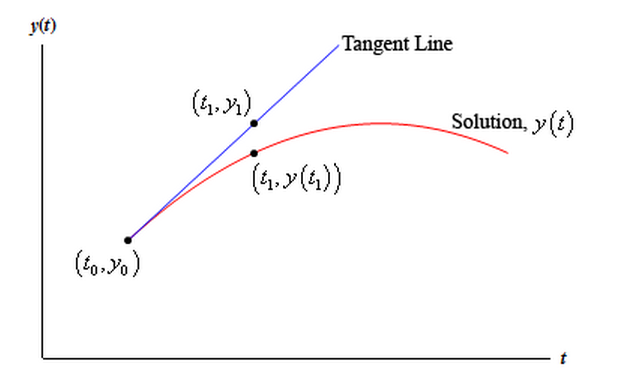
\includegraphics[width=0.65\textwidth]{figures/tangent_line_approx.png}
   \caption{ Tangent line Approximation }
\end{figure}


\paragraph{}
Note that since we are given $f(t,y)$ as well as the point $(t_0,y_0)$, $f(t_0,y_0)$ is a constant, as is $f(t_0,y_0)t_0 + y_0$ .  So we have an equation in the form of $y_1=mt_1+b$. Now, Let's pick a value for $t_1$ that is relatively close to $t_0$ and plug it into our point-slope equation to solve for $y_1$.
\paragraph{}
 We can take our new point $(t_1,y_1)$ and plug them into our given equation $ \dfrac{dy}{dt}=f(t,y)$ in order to find the slope of the line that is tangent to our solution at $(t_1,y_1)$. We can then take that slope and use it to create a line that is parallel to the line that is tangent to our solution, but passes through our known point $(t_1,y_1)$. 
\[
\frac{dy}{dt} = f(t_1,y_1)
\] 
\[
y_2 - y_1 = f(t_1,y_1)(t_2 - t_1) 
\]
Once again, we have the equation of a line in the form of 
\[
y_2 = mt_2+b
\]
See figure 2 for a graphical representation of what we just did.

\begin{figure}[H]
  
  \centering
   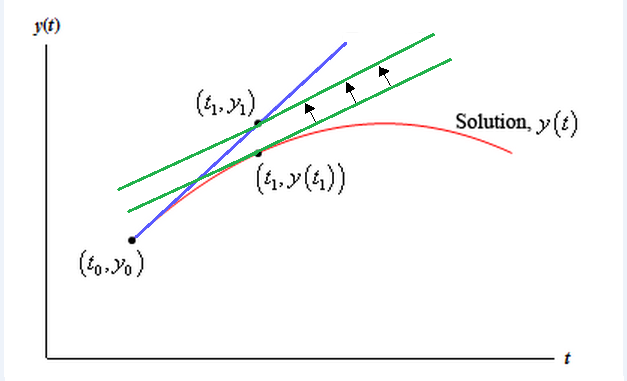
\includegraphics[width=0.65\textwidth]{figures/TLA2}
   \caption{ Adding Another Line with the same slope as the line tangent to the solution, but going through the known point $(t_1,y_1)$}
\end{figure}


Hopefully you can see where this is going. We can continue this process and end up with something that looks like this:

\begin{figure}[H]
  \centering
   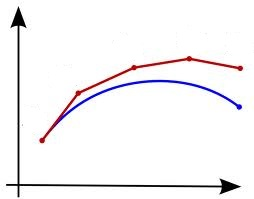
\includegraphics[width=0.5\textwidth]{figures/TLA3}
 
\end{figure}

We can take this process one step further by creating a recursive function. 
\[
t_{n+1} = y_n + f(t_n,y_n)(t_{n+1} - t_n) 
\]  
Now, we should pick some constant $h$ that defines the difference between $t_{n+1}$ and $t_n$ So that for every iteration of our recursive function, $t$ is incremented uniformly. So 
\[
h = t_{n+1} - t_n
\] 
and 
\[
t_{n+1} = y_n + f(t_n,y_n)h
\]
finally, we can create a short hand for $f(t_n,y_n)$, $f_n$.
\[
y_{n+1} = y_n + f_nh
\]

\section*{Example}
\subsection*{Disclaimer}

This example is going to get somewhat in-depth. However, I feel as though I would be doing a disservice to my fellow math enthusiasts if i did not fully exemplify the beauty Euler's method.
\subsection*{Let's Do This!} 
Consider the differential equation $y'= 1-t+y$
where $y(t_0) = y_0$. First, you may notice that it is in the form of $y' +p(t)y = g(t)$, so let's solve it by analytic means so that we have a known answer to work towards.
\[
\frac{dy}{dt} - y = 1-t
\]
\[
p(t) = -1
\]
\[
\mu(t) = \exp{\int {-1} ,dt}
\]
\[
\mu(t) = e^{-t}
\]
\[
e^{-t}\frac{dy}{dt} - ye^{-t}= e^{-t}(1-t)
\]
\[
\frac{d}{dt}\left[e^{-t}y\right] = e^{-t}-te^{-t}
\]
\[
e^{-t}y = \int{(e^{-t}-te^{-t})}dt + C
\]
\[
e^{-t}y = \int {e^{-t}}dt - \int {te^{-t}} dt +C 
\]
Integration By Parts
\[
\int {te^{-t}} dt  = -te^{-t} + \int{e^{-t}}dt
\]
\[
e^{-t}y = -e^{-t} + te^{-t} + e^{-t} + C
\]
\[
e^{-t}y = te^{-t}  + C
\]
\[
y = t + Ce^t
\]
\[
y_0 = t_0 +Ce^{t_0}
\]
\[
C = \frac{y_0 - t_0}{e^{t_0}}
\]
\[
y= t + \left(  \frac{y_0 - t_0}{e^{t_0}} \right)e^t
\]
\[
y= t + (y_0 - t_0)e^{t-t_0}
\]
Now, Let's see what happens when we apply Euler's method to this differential equation.
\[
f(t,y) = 1 - t + y
\] 
\[
y_{n+1} = y_n + f_nh
\]


\subsection*{Tangent For CS Enthusiasts (Get it? Tangent!)}
We are going to try to write a program that will approximate this differential equation. If you are not interested in coding or do not understand it, that's fine. You can just skip this section. Otherwise, Enjoy! 

\paragraph{}
The first thing we need to do is create a function that models our given function, $f(t,y)$. 
We'll call our function F, which takes two parameters: t and y, and returns 1-t+y. Our second function will call on f and will implement a for loop to pass $t_n$ and $y_n$ as arguments to F.  This function will take the perimeters $t_0$ and $y_0$.   
 

 \begin{algorithmic}
\Function{f}{$t$,$y$}
\State \Return $1-t+y$
\EndFunction 
 
 
\Function{Print Data}{$t_0$, $y_0$}
\State Initialize $t_n \gets t_0$ 
 \State Initialize $y_n \gets y_0$ 
 \State Initialize $t_{n+1} \gets 0 $
 \State Initialize $y_{n+1} \gets 0$
 \State print $t_n$ and $y_n$ to a file separated by a comma.
 \State print a new line to the file

 
\For{$i:=n \to N$}
\State $t_{n+1} \gets t_n + h$
\State $y_{n+1} \gets \Call{f}{t_n,y_n}t_{n+1} - \Call{f}{t_n,y_n} t_n +y_n$
\State print $y_{n+1}$ and $t_{n+1}$ to a file separated with a comma
\State print a new line to the file
\State $t_n \gets t_{n+1}$
\State $y_n \gets y_{n+1}$
\EndFor

\EndFunction
	
\end{algorithmic}
 
\paragraph{}
I ran this program for the initial value of $y(0)=1$. I set $h = . 1$ and $1<i<50$ and plotted the data in a Microsoft Excel line graph along with the actual solution of $y = t + e^t$. I also ran the program with $h = .05$ and $1<n<100$ to show that our approximation becomes more precise as $h \to 0$.

\begin{figure}[H]
\begin{subfigure}{0.5\textwidth}
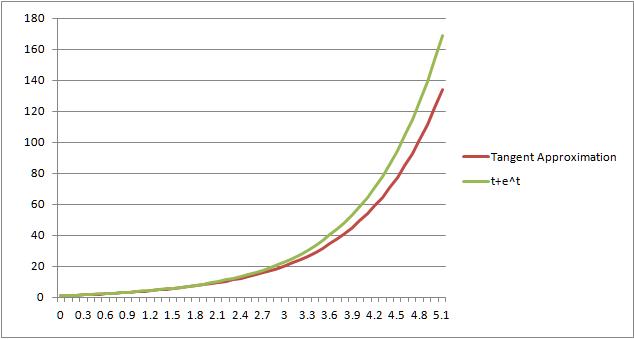
\includegraphics[width=.75\textwidth]{figures/excell_data}
\caption
{
Tangent line approximation vs. solution with $h= .1$ 
}
\end{subfigure}~\quad
\begin{subfigure}{.5\textwidth}
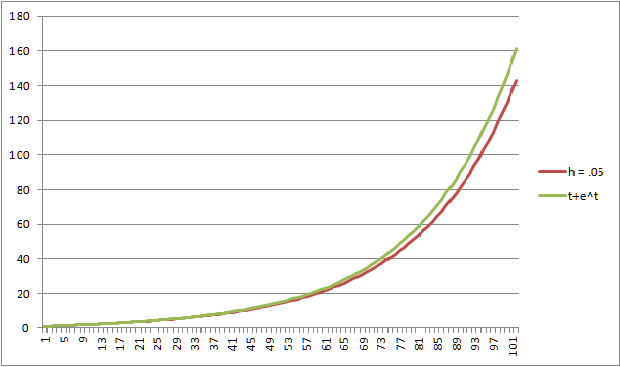
\includegraphics[width=.75\textwidth]{figures/excell_data2}
\caption
{
Tangent line approximation vs solution when $h = .05$. 
}
\end{subfigure}
\end{figure}




\subsection*{Finding a Closed Form for Our Equation }

\paragraph{}
Now, here is where things get interesting. We are going to attempt to find a closed form for our recursive function. Wikipedia: In mathematics, an expression is said to be a closed-form expression if it can be expressed analytically in terms of a finite number of certain "well-known" functions. In other words, we want to find an expression for our function so that we can find the value of the function for any given $n$ without having to iterate through every proceeding value of $n$.
 
\paragraph{}
Let's start with Euler's Equation.
\[
y_{n+1} = y_n + f_nh
\]
and our equation 
\[
f(t,y) = 1 - t +y, y(t_0) = y_0
\]
so 
\[
y_{1} = y_0 + (1-t_0+y_0)h
\]
distributing the $h$
\[
y_1 = y_0 + hy_0 +h -ht_0
\]
pulling out a $y_0$
\[
y_1 = y_0(1+h) +h - ht_0
\]
but since we know that $t_1 = t_0+h$, we can do an interesting trick.
\[
y_1 = y_0(1+h) +h -ht_0 -t_1+t_1 
\]
\[
y_1 = y_0(1+h) +h -ht_0 -h-t_0 +t_1
\]
\[
y_1 = y_0(1+h) -ht_0-t_0+t_1
\]
factoring out a $-t_0$
\[
y_1 = y_0(1+h) -t_0(1+h)
\]
factoring out a $(1+h)$
\[
y_1 = (1+h) (y_0-t_0) + t_1
\]
Now, let's take our expression for $y_1$ and see what happens when we try to find $y_2$
\[
y_2 = (1+h)(y_1-t_1) + t_2
\]
\[
y_2 = (1+h)\left[(1+h)(y_0-t_0)+ t_1 - t_1\right]	 + t_2
\]
\[
y_2=(1+h)^2(y_0-t_0)+t_2
\]
Hopefully you can see the pattern here. It looks as if 
\[
y_n=(1+h)^n(y_0-t_0)+t_n
\]
However, we only have a hunch that this is the pattern that we are dealing with. We must now prove my the method of induction that our guess is correct.
\paragraph{}
So, we are going to assume that $y_n=(1+h)^n(y_0-t_0)+t_n$ is true and plug that into our base case.
\[
y_{n+1} = (1+h) (y_n-t_n) + t_{n+1}
\]
\[
y_{n+1} = (1+h) \left[(1+h)^n(y_0-t_0)+t_n -t_n\right] + t_{n+1}
\]
\[
y_{n+1} = (1+h)^{n+1}(y_0-t_0)+t_{n+1}
\]
\[ 
y_n = (1+h)^n(y_0-t_0)+t_n
\] 
Success! Our guess was right. We now have a closed form for our recursive function that that will give us the value of $y_n$ for any given $n$.

\subsection*{We're Almost There}
Now, we can show that the closed form of our expression will, in fact, converge to our solution, $y= t + (y_0 - t_0)e^{t-t_0}$ as $n \to \infty.$
\paragraph{}
The fist thing we need to is is pick some value for h. For this example, we are going to pick
\[
h = \frac{t-t_0}{n}
\]
so as $n \to \infty$, $h \to 0$ .\\\\
Now, let's see what happens to $y_n$ as $n \to \infty.$
\[
\lim_{n \to \infty} y_n = \lim_{n \to \infty}  (1+\frac{t-t_0}{n})^n(y_0-t_0)+t_n
\]
For the sake of simplicity, Let substitute $T$ for $t-t_0$. We also know that since $(y_0-t_0)+t_n$ is a constant, it won't be significant at infinity. So we are going to set
\[
\phi = (1+\frac{T}{n})^n
\]
\[
\lim_{n \to \infty} \phi  = \lim_{n \to \infty}  (1+\frac{T}{n})^n
\]
\[
\ln \lim_{n \to \infty} \phi  = \ln \lim_{n \to \infty}  (1+\frac{T}{n})^n 
\]
 \[
 \ln \lim_{n \to \infty} \phi  = \lim_{n \to \infty}  n\ln (1+\frac{T}{n}) 
 \]
 \[
 \ln \lim_{n \to \infty} \phi  = \lim_{n \to \infty}  \frac{\ln (1+\frac{T}{n})}{\frac{1}{n}}
 \]
  l'Hôpital's rule
  \[
 \ln \lim_{n \to \infty} \phi  = \lim_{n \to \infty}  \frac{\frac{1}{1+\frac{T}{n}}\left(\frac{-T}{n^2}\right)}{\frac{-1}{n^2}}  
  \]
  \[
 \ln \lim_{n \to \infty} \phi  = \lim_{n \to \infty}  \frac{T}{1+\frac{T}{n}}  
  \]
  \[
  \ln \phi = T
  \]
  \[
  \phi = e^{t-t_0}
  \]
  \[
  \lim_{n\to\infty}y_n = e^{t-t_0}(y_0-t_0)+t 
  \]
does that expression look familiar?

\chapter{Second order Differential Equations}
\section{Finding the characteristic Equation}
\subsection*{A few words on notation}
\paragraph{}
If we were to see the expression $f(x) = 3x^2+x$ we would say that we have a function called $f$, which takes one parameter, $x$, raises it to the power of $2$, multiplies it by $3$, and then adds the original parameter. We could also say that $f$ is an operator. There is another operator used in differential equations called the ``differential operator". This operator is denoted by $L[\phi]$, and instead of taking a variable as a parameter, it takes a function, $\phi$.
\paragraph{}
The formal definition of this operator goes like this:\\
Let $p(t)$ and $q(t)$ be continuous functions on an open interval $I: \alpha<t<\beta $, then for any function $\phi$ that is twice-differentiable on $I$, we define the differential operator $L$ by the equation 
\[
L[\phi] = \phi'' + p\phi' +q\phi
\] 
and the value of $L$ at point $t$ is 
\[
L[\phi](t) = \phi''(t) + p(t)\phi'(t) +q(t)\phi(t)
\]

\subsection{Homogeneous Equations}
\paragraph{}
A homogeneous equation is one that is in the form 
\[
p(t)y''+q(t)y'+r(t)y =0
\]
or
\[
L[\phi](t) = 0
\]
A homogeneous equation with constant coefficients is one in the form of 
\[
ay''+by'+cy = 0
\]
 this expression can also be written as 
\[
L[y] = 0
\]
where $p = \dfrac{b}{a}$ and $q = \dfrac{c}{a}$\\
\paragraph{}
Let's see if we can't guess a solution to this differential equation.
\[
y = e^{rt}
\]
\[
y' = re^{rt}
\]
\[
y'' = r^2e^{rt}
\]
\[
ay''+by'+cy = ar^2e^{rt}+bre^{rt} +ce^{rt} = 0
\]
factoring out a $e^{rt}$
\[
ar^2+br + c = 0
\]
This is called the "characteristic equation". We can use the quadratic formula to find two possible values of $r$
\[
r_1 = \frac{-b + \sqrt{b^2-4ac}}{2a}
\]
\[
r_2 = \frac{-b - \sqrt{b^2-4ac}}{2a}
\]
so we have two possible solutions:
\[
y_1 =  e^{r_1t}
\]
\[
y_2 = e^{r_2t}
\]
Now, we can prove that our result is, in fact, a solution to the differential equation.
\[
y = e^{rt}
\]
\[
y' = re^{rt}
\]
\[
y'' = r^2e^{rt}
\]
Our original equation
\[
ay''+by'+cy = 0
\]
Plugging in our solution
\[
ar^2e^{rt} +bre^{rt}+c{rt} = 0
\]
\[
ar^2 + br+ c = 0
\]
and since we have found an $r$ that makes this equation equal to $0$, we know that both of our solutions are correct.\\
\paragraph{•}
Since 
\[
y_1 =  e^{r_1t}\quad \text{and} \quad y_2 = e^{r_2t}
\]
are both solutions, it follows that 
\[
C_1y_1 =  C_1e^{r_1t}\quad \text{and} \quad C_2y_2 = C_2e^{r_2t}
\]
are also solutions.
\paragraph{•} 
So we have proven than for any differential equation in the form of 
\[
ay''+by'+cy = 0
\]
at least two solutions are
\[
y_1 = C_1 e^{r_1t}
\]
and
\[
y_2 = C_2e^{r_2t}
\]

\subsection{The Superposition Principle}
Recall that a homogeneous equation is one that is in the form of 
\[
L[\phi] = \phi'' + p\phi' +q\phi= 0
\] 
we have just proven that $y_1$ and $y_2$ are solutions to any homogeneous equation. So 
\[
L[y_1] = y_1'' +py_1'+qy_1 = 0
\]
and 
\[
L[y_2] = y_2''+py_2'+qy_2 = 0
\]
Now, we can prove that $y_1+y_2$ is also a solution. So
\begin{equation*}
L[y_1+y_2] = [y_1+y_2]'' + p[y_1+y_2 ]' + q [y_1+y_2]
\end{equation*}
\begin{align*}
 &= y_1''+y_2'' + py_1'+py_2' + qy_1+qy_2 \\
 &= y_1''+ py_1'+qy_1+y_2''+py_2'+qy_2 \\
  &= L[y_1]+ L[y_2]
\end{align*}

$L[y_1]$ and $L[y_2]$ are equal to $0$, therefore $L[y_1+y_2]$, therefore $y_1+y_2$ is a solution. So our assumption was correct.
So we have proven that for any homogeneous equation with constant coefficients, a solution is 
\[
y = C_1 e^{r_1t}+C_2e^{r_2t}
\] 
 Now, let's see what happens when we attempt to find a particular solution to a homogeneous equation with constant coefficients if we are given the initial values $y(t_0) = y_0$ and $y'(t_0) = y'_0$. 
 \subsection{Wronskian Determinant}
 \paragraph{•}
 We know that for any homogeneous differential equation with constant coefficients $y = C_1 e^{r_1t}+C_2e^{r_2t}$ or $y = y_1 + y_2$ is a solution. So if we are given the initial value conditions $y(t_0) = y_0$ and $y'(t_0) = y'_0$ we can set 
 \[
 y_0 = y_1(t_0) + y_2(t_0)
 \]
 and
 \[
 y_0' = y_1'(t_0) + y_2'(t_0)
 \]
 Now, we treat these two expressions as a system of equations and take the Wronskian Determinant. 
 \[
 W[y_1(t_0),y_2(t_0)] =
 \begin{vmatrix}
 y_1(t_0) & y_2(t_0)\\
 y_1'(t_0) & y_2'(t_0)
 \end{vmatrix} 
 = y_1(t_0)y_2'(t_0)-y_2(t_0)y_1'(t_0)
 \]
 If $W \neq 0 $, then $y_1$ and $y_2$ form a fundamental set of solutions.
 \subsection*{Example}
 \[
 y'' + 4y' +3y = 0;\quad
 y(0) = 2, \quad y'(0) = -1
 \] 
 \[
 r^2 + 4r+3 = 0 
 \]
\[
(r+3)(r+1) = 0
\]
\[
r = -3\quad r = -1
\]

so
\[
y = C_1y_1 + C_2y_2
\]
where 
\[
y_1 =  e^{-3t}\quad\text{and}\quad y_2 = e^{-t}
\]
similarly 
\[
y' = C_1y_1' + C_2y_2'
\]
where 
\[
y_1' = (-3) e^{-3t}\quad\text{and}\quad
y_2' = -e^{-t}
\]
Now we take the Wronskain determinant.
\[
W[y_1(t_0),y_2(t_0)] = 
\begin{vmatrix}
1&1\\
-3&-1
\end{vmatrix}
= -1+4 = 3 \neq 0 
\]
so we know that a solution exists. So we can solve the system of equations 
\[
C_1 + C_2 = 2
\]
\[
-3C_1 - C_2 = -1
\]
\[
C_1 = -\frac{1}{2}\quad\text{and}\quad C_2 = \frac{5}{2}
\]
so 
\[
y = \frac{5}{2}e^{-t} - \frac{1}{2}e^{-3t}
\]
\subsection*{Theorem}
\paragraph{}
Recall that $W[y_1(t_0),y_2(t_0)] = y_1(t_0)y_2'(t_0)-y_2(t_0)y_1'(t_0) $
Now, say we were given a second order linear homogeneous differential equation with the initial value of $t_0$, but no $y_0$ or $y'_0$. We can use the Wronskian Determinant to to pick an initial condition that will be guaranteed to give a fundamental set of solutions. We can do this by picking a $y_1(t_0)$, $y_2(t_0)$,$y_1'(t_0)$, and $y_2'(t_0)$ such that $y_1(t_0)y_2'(t_0)-y_2(t_0)y_1'(t_0) > 0 $
\[
y_1(t_0) = 1 \quad y_2'(t_0) = 1
\]
\[
y_2(t_0) = 0 \quad y_1'(t_0) = 0
\]
this way 
\[
\begin{vmatrix}
1 & 0 \\
0 & 1
\end{vmatrix}
= 1
\]
\subsection{Abel's Theorem}
\paragraph{•}
Suppose that 
\[
y_1'' + p(t)y_1' + q(t)y_1 = 0 
\]
and
\[
y_2'' + p(t)y_2' + q(t)y_2 = 0 
\]
if we multiply the first equation by $-y_2$ and the second by $y_1$ we get
\[
-y_2y_1'' - p(t)y_2y_1' - q(t)y_2y_1 = 0 
\]
\[
y_1y_2'' + p(t)y_1y_2' + q(t)y_1y_2 = 0 
\]
setting these two equation equal to each other and grouping terms we get 
\[
(y_1y_2''-y_2y_1'') + p(t)(y_1y_2'-y_2y_1') = 0
\] 
Now we take the Wronskian of $y_1$ and $y_2$
\[
W[y_1,y_2] = 
\begin{vmatrix}
y_1 & y_2\\
y_1' & y_2'
\end{vmatrix}
= y_1y_2'-y_2y_1'
\]
so 
\[
W'[y_1,y_2] = y_1'y_2'+y_2''y_1 - (y_2'y_1'+y_1''y_2)
\]
\[
W'[y_1,y_2] = y_2'' y_1 - y_1''y_2
\]
so 
\[
W'[y_1,y_2] + p(t)W[y_1,y_2] = 0
\]
\[
W'  = -p(t)W
\]
this is a separable equation that we can easily solve 
\[
W = C\exp\left[-\int{p(t)}dt\right]
\] 
\section{Complex Roots}
\subsection{Taylor Series}
\paragraph*{•}
In order to fully understand the idea behind this section, we must fist do a small review of the Taylor Series and Maclaurin Series.
\paragraph*{}
The idea behind the Maclaurin Series is that if we have some function, we can approximate that function about a certain interval by building a polynomial whose derivatives match those the function's at 0. In other words, if we have some function $f$ that is differentiable at $0$ we can call our approximation $P$. So
\begin{align*}
&P(0) = f(0)\\
&P'(0) = f'(0)\\
&P''(0) = f''(0)\\
&...\\
&P^{(n)}(0) = f^{(n)}(0)
\end{align*}
and we can build a polynomial that looks like
\[
p(x) \approx f(0) + f'(0)x + \frac{f''(0)}{2}x^2 + \frac{f'''(0)}{6}x^3 +....+ \dfrac{f^{n}(0)}{n!}x^n
\]
So we get something that looks like this.
\begin{figure}[H]
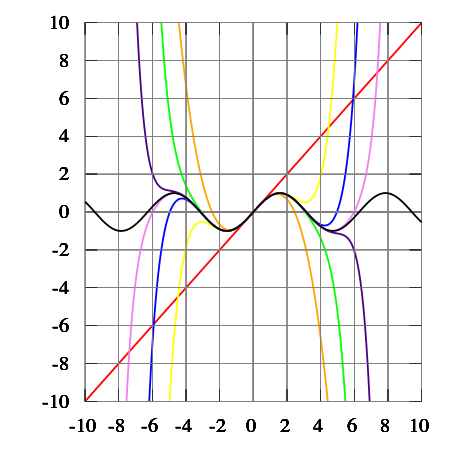
\includegraphics[width=0.45\textwidth]{figures/Taylor}
\end{figure}
\paragraph{}
The Taylor Series simply takes this idea and expands it work for points other than $0$.
Sometimes, the series will converge about an interval, sometimes it will converge for all $x$,  sometimes it will not converge at all. There are numerous tests to determine whether a series converges, but that is not important for this chapter. We need only to know that there are three particular series which converge for all x: 
\[
e^x, \quad \cos(x) , \quad  \text{and} \quad \sin(x)
\]
and their Taylor expansions look like this 
\[
e^x \approx 1 + x + \frac{x^2}{2} + \frac{x^3}{3!} +\frac{x^4}{4!}+....+ \frac{x^n}{n!}
\]
\[
\cos(x) \approx 1 - \frac{x^2}{2} + \frac{x^4}{4!} - \frac{x^8}{8!} + \frac{x^{10}}{10!} +.....+\frac{(-1)^{n}x^{2n}}{2n!}
\]
\[
\sin(x) \approx x - \frac{x^3}{3!} + \frac{x^5}{5!} - \frac{x^7}{7!} + \frac{x^9}{9!} +....+ \frac{(-1)^nx^{2n+1}}{(2n+1)!}
\]
\subsection{Euler's Equation}
Now, what happens if we were to take $e^{it}$?
\begin{align*}
e^{ix} &\approx 1 + ix + \frac{(ix)^2}{2} + \frac{(ix)^3}{3!} +\frac{(ix)^4}{4!}+...\\
&= 1 + ix - \frac{x^2}{2}- \frac{ix^3}{3!}+\frac{x^4}{4!}+\frac{ix^5}{5!}
\end{align*}
now, Let's group the real and the complex terms together.
\[
e^{ix} \approx (1 - \frac{x^2}{2} +\frac{x^4}{4!} +....) + i(x-\frac{(x)^3}{3!}+\frac{(x)^5}{5!}+....)
\]
\[
e^{ix} \approx \cos(x) + i\sin(x)
\]
as it turns out, this series also converges for all $x$, so 
\[
e^{ix} = \cos(x) + i\sin(x)
\]
\subsection{Relating this to Differential Equations}
A few identities that we should know(you can test these out for yourself):
\begin{align*}
&e^{-it} = \cos(t) - i\sin(t)\\
&e^{\mu it}=\cos(\mu t) + i\sin(\mu t)
\end{align*}
We also know that
\begin{align*}
e^{(\sigma + i \mu )t} &= e^{\sigma t}e^{i\mu t}\\
& = e^{\sigma t}(\cos(\mu t) + i\sin(\mu t))\\
&= e^{\sigma t}\cos(\mu t)+ i e^{\sigma t}\sin(\mu t)
\end{align*}
Let's set  $e^{\sigma t}\cos(\mu t) = u(t)$ and $e^{\sigma t}\sin(\mu t) = v(t)$\\\\
so 
\[
e^{\sigma + i \mu t} = u(t) + iv(t)
\]
Let's assume that $y =  u(t) + iv(t)$ is a solution to a homogeneous linear second order differential equation. So 
\[
L[y] = 0
\]
\[
u''(t) + iv''(t) + p(t)[u'(t) + iv'(t)] + q(t)[u(t) + iv(t)] = 0
\]
\[
(iv''(t) + p(t)iv'(t) + q(t) iv(t)) + (u''(t) + p(t)u'(t) + q(t) u(t)) = 0
\]
pulling out an $i$ from the left side 
\[
i[v''(t) + p(t)v'(t) + q(t) v(t)] + u''(t) + p(t)u'(t) + q(t) u(t) = 0
\]
\[
iL[v](t) + L[u](t) = 0
\]
\[
L[v](t) \quad \text{and} \quad L[u](t) = 0
\]
so $v(t)$ and $u(t)$ are solutions to the equation.\\\\
Taking the Wronskian Determinant 
\[
W[u(t), v(t)] = \mu e^{2\sigma t}
\] 
so as long as $\mu \neq 0$, $u(t)$ and $v(t)$ are a fundamental set of solutions
Furthermore, by the superposition principle 
\begin{align*}
y &= v(t) + u(t)\\
&= e^{\sigma t}\cos(\mu t) + e^{\sigma t}\sin(\mu t)
\end{align*}


So if we are given a homogeneous second order differential equation whose solutions come in the form of 
\[
y_1 = c_1\exp[(\sigma + i \mu) t]
\]
and 
\[
y_2 = c_2\exp[(\sigma - i \mu) t],
\]
then
\[
y_1 = c_1e^{\sigma t}\cos(\mu t) + c_1e^{\sigma t}\sin(\mu t)
\]
and 
\[
y_2 = c_2e^{\sigma t}\cos(\mu t) - c_2e^{\sigma t}\sin(\mu t).
\]
So 
\begin{align*}
y = c_1y_1 + c_2y_2 &= c_1e^{\sigma t}\cos(\mu t) + c_1e^{\sigma t}\sin(\mu t) + c_2e^{\sigma t}\cos(\mu t) - c_2e^{\sigma t}\sin(\mu t)\\
&= e^{\sigma t}\cos(\mu t)[c_1+c_2]+ e^{\sigma t}\sin(\mu t)[c_1-c_2]
\end{align*}
renaming our constants, we get
\[
y = c_1e^{\sigma t}\cos(\mu t)+ c_2e^{\sigma t}\sin(\mu t).
\]




\section{Repeated Roots}

Say we are given a homogeneous differential equations with constant coefficients. We find the characteristic equation and solve for $r$. So
\[
ar^2+br + c = 0
\]
\[
r = -b \pm \frac{\sqrt{b^2-4ac}}{2a}.
\]
But than we run into a problem, 
\[
b^2-4ac=0.
\]
This means that we can find one solution to the differential equation,
\[
y_1= \exp\left[\frac{-b}{2a}\right]
\]
but we must still find the other solution in order to find the fundamental set of solutions.
\paragraph{}
So let's assume that 
\begin{align*}
y &= v(t)y_1(t)\\
&= v(t)\exp\left[\frac{-b}{2a}\right]
\end{align*}
\begin{align*}
y'(t) = v'(t)\exp\left[\frac{-b}{2a}\right] -\frac{b}{2a}v(t)\exp\left[\frac{-b}{2a}\right]
\end{align*}
\begin{align*}
y''(t) &= v''(t)\exp\left[\frac{-b}{2a}\right] -\frac{b}{2a}v(t)\exp\left[\frac{-b}{2a}\right] - \left[ \frac{b}{2a}v'(t)\exp\left[\frac{-b}{2a}\right] -\frac{b^2}{4a^2}v(t)\exp\left[\frac{-b}{2a}\right]  \right]\\
&=  v''(t)\exp\left[\frac{-b}{2a}\right] -\frac{b}{2a}v(t)\exp\left[\frac{-b}{2a}\right] -  \frac{b}{2a}v'(t)\exp\left[\frac{-b}{2a}\right] +\frac{b^2}{4a^2}v(t)\exp\left[\frac{-b}{2a}\right]\\
&=  v''(t)\exp\left[\frac{-b}{2a}\right] -\frac{b}{a}v'(t)\exp\left[\frac{-b}{2a}\right]  +\frac{b^2}{4a^2}v(t)\exp\left[\frac{-b}{2a}\right]  
\end{align*}

Plugging these identities into the given differential equation.
\begin{align*}
&a \left(     v''(t)\exp\left[\frac{-b}{2a}\right] -\frac{b}{a}v'(t)\exp\left[\frac{-b}{2a}\right]  +\frac{b^2}{4a^2}v(t)\exp\left[\frac{-b}{2a}\right]   \right)\\
 + &b \left(  v'(t)\exp\left[\frac{-b}{2a}\right] -\frac{b}{2a}v(t)\exp\left[\frac{-b}{2a}\right] \right)\\
  + &cv(t)\exp\left[\frac{-b}{2a}\right]= 0
  \end{align*}

\begin{align*}
    av''(t)-bv'(t) +\frac{b^2}{4a}v(t) + bv'(t)-\frac{b^2}{2a}v(t) + cv(t) = 0  
\end{align*}
\[
av''(t) +(-b+b)v'(t) + \left(   \frac{b^2}{4a} - \frac{b^2}{2a} + c  \right)v(t) = 0
\]
\[
av''(t) +\left(	\frac{-b^2}{4a} + c	\right)v(t) = 0
\]
Now, let's take a look at the expression 
\[
\frac{-b^2}{4a} + c.
\]
this can be rewritten as 
\[
\frac{4ac-b^2}{4a}
\]
We know that 
\[
b^2-4ac = 0
\]
\[
b^2 = 4ac
\]
so 
\[
\frac{4ac-b^2}{4a} = 0
\]
so 
\[
v''(t) = 0
\]
\[
v'(t) = c
\]
\[
v(t) = c_1t+c_2
\]
and finally 
\begin{align*}
y &= \left(  c_1t +c_2 \right)\exp\left[	\frac{-bt}{2a}	\right]\\
&= c_1t\exp\left[	\frac{-bt}{2a}	\right] + c_2\exp\left[	\frac{-bt}{2a}	\right]
\end{align*}
and by the superposition principle 
\[
y_1 =  c_1t\exp\left[	\frac{-bt}{2a}	\right]
\]
\[
y_2 = c_2\exp\left[	\frac{-bt}{2a}	\right]
\]
Taking the Wronskian determinant 
\[
W[y_1,y_2] = \exp{\frac{-bt}{a}},
\]
which will never equal 0. So 
$y_1$ and $y_2$ form a fundamental set of solutions.


\section{Euler Equations}
\paragraph{}
Consider an equation in the form 
\[
t^2 \frac{d^2y}{dt^2} + \alpha t\frac{dy}{dt} + \beta y = 0
\]
Let $x$ = $\ln t$ 
\begin{align*}
\frac{dy}{dt} &= \frac{dy}{dx} \frac{dx}{dt}\\
&= \frac{dy}{dx}\frac{1}{t}\\\\
\frac{d}{dt}\left[\frac{dy}{dt}\right] 
&= \frac{d}{dt}\left[\frac{dy}{dx}\right]\frac{1}{t}-\frac{dy}{dx}\frac{1}{t^2}\\
\frac{d^2y}{dt^2}&= \frac{d^2y}{dx^2}\frac{1}{t^2}- \frac{dy}{dt}\frac{1}{t^2}
\end{align*}

Plugging these identities into our original equation 
\[
\frac{d^2y}{dx^2}-\frac{dy}{dx} + \alpha\frac{dy}{dx}+\beta y = 0
\]
\[
\frac{d^2y}{dx^2}+\frac{dy}{dx}\left(\alpha - 1\right)+\beta y = 0
\]
or
\[
y''+y'(\alpha-1) + \beta y = 0
\]
This is a linear homogeneous equation that can be solved by methods previously stated.

\section{ Non-homogeneous equations}
\subsection{Cramer's Rule}
\paragraph{}
Consider the system of equations 
\begin{align*}
ax+by &= e\\
cx+dy &= f
\end{align*}
Cramer's Rule states that 
\[
x = \frac{
\begin{vmatrix}
e&b\\
f&d
\end{vmatrix}
}{
\begin{vmatrix}
a&b\\
c&d

\end{vmatrix}
}
\quad \quad \quad
y = \frac{
\begin{vmatrix}
a&e\\
c&f
\end{vmatrix}
}{
\begin{vmatrix}
a&b\\
c&d

\end{vmatrix}
}
\]

\subsection{Variation of Parameters}
\paragraph*{}
Consider the second order linear non-homogeneous differential equation in the form of 
\[
y''+p(t)y'(t)+q(t)y(t) = g(t)
\] 
We are going to assume that the homogeneous equation 
\[
y''+p(t)y'(t)+q(t)y(t) = 0 
\]
can be solved by analytic means. So
\[
y = c_1y_1+c_2y_2 
\]
is the solution to this homogeneous equation; furthermore,  $y_1$ and $y_2$ form a fundamental set of solutions.
\paragraph{•}
We are going to replace $c_1$ and $c_2$ with functions of $t$, $u_1(t)$ and $u_2(t)$. 
So
\[
y = u_1(t)y_1(t) + u_2(t)y_2(t)
\]
\[
y' = u_1'(t)y_1(t) + u_1(t)y_1'(t) + u_2'(t)y_2(t) + u_2(t)y_2'(t)
\]
We are going to set 
\[
 u_1'(t)y_1(t) + u_2'(t)y_2(t) = 0.
\]
If at this point you are beginning to feel skeptical, that's a good thing! We have not yet proven that this will always be the case. However, we will make this assumption for now and see how it affects the outcome later on. So we have
\[
y' = u_1(t)y_1'(t) +  u_2(t)y_2'(t)
\]
\[
y'' = u_1'(t)y_1'(t)+u_1(t)y_1''(t) +  u_2'(t)y_2'(t) + u_2(t)y_2''(t)
\]
 plugging these identities into our original equation, we get
 \[
  y''+p(t)y'(t)+q(t)y(t) = g(t)\\
  \]
  \begin{align*}
  &u_1'(t)y_1'(t)+u_1(t)y_1''(t) +  u_2'(t)y_2'(t) + u_2(t)y_2''(t)\\
  +  &p(t)[u_1(t)y_1'(t) +  u_2(t)y_2'(t)] \\
  + &q(t)[u_1(t)y_1(t) + u_2(t)y_2(t)] = g(t)
\end{align*}
Distributing the $p(t)$ and $q(t)$ we get
\begin{align*}
&u_1'(t)y_1'(t)+u_1(t)y_1''(t) +  u_2'(t)y_2'(t) + u_2(t)y_2''(t)\\
  + &p(t)u_1(t)y_1'(t) +p(t)u_2(t)y_2'(t)\\ 
  + &q(t)u_1(t)y_1(t)+q(t)u_2(t)y_2(t) = g(t).
\end{align*}
Grouping terms we get
\begin{align*}
&u_1(t)[y_1''(t)+p(t)y_1'(t)+q(t)y_1(t)]\\
+ &u_2(t)[y_2''(t)+p(t)y_2'(t)+y_2(t)]\\
+ &u_1'(t)y_1'(t) + u_2'(t)y_2'(t) = g(t).
\end{align*}
 However, 
 \[
 y_1''(t)+p(t)y_1'(t)+q(t)y_1(t) \quad \text{and} \quad y_2''(t)+p(t)y_2'(t)+y_2(t)
 \]
are both equal to zero, because $y_1$ and $y_2$ are solution to to the homogeneous equation 
\[
y''+p(t)y'(t)+q(t)y(t) = 0 ,
\]
So we have 
 \[
  u_1'(t)y_1'(t) + u_2'(t)y_2'(t) = g(t).
 \]
 Recall that we have made the assumption that 
 \[
 u_1'(t)y_1(t) + u_2'(t)y_2(t) = 0.
 \]
 We now have a system of equations.
 \[
 u_1'(t)y_1'(t) + u_2'(t)y_2'(t) = g(t)
 \]
\[
 u_1'(t)y_1(t) + u_2'(t)y_2(t) = 0
\] 
 Now we can use Cramer's Rule 
 \[
 u_1'(t) = \frac{
\begin{vmatrix}
g(t)&y_2'(t)\\
0&y2(t)
\end{vmatrix}
}{
\begin{vmatrix}
y_1'(t)&y_2'(t)\\
y_1(t)&y_2(t)
\end{vmatrix}
}
= \frac{g(t)y_2(t)}{-W[y_1,y_2](t)}
\quad \quad \quad
u_2'(t) = \frac{
\begin{vmatrix}
y_1'(t)&g(t)\\
y_1(t)&0
\end{vmatrix}
}{
\begin{vmatrix}
y_1'(t)&y_2'(t)\\
y_1(t)&y_2(t)
\end{vmatrix}
}
= \frac{g(t)y_1(t)}{W[y_1,y_2](t)}
 \]
 Recall that $y_1$ and $y_2$ form a fundamental set of solutions, so $W[y_1,y_2] \neq 0$.
\[
u_1(t) = - \int{\frac{g(t)y_2(t)}{W[y_1,y_2](t)}dt}
\quad \quad
u_2(t) = \int{\frac{g(t)y_1(t)}{W[y_1,y_2](t)}dt}
\]
\subsection{Yet Another Theorem Brought to Us by Euler}
For any second order linear non-homogeneous differential equation in the form of 
\[
y''+p(t)y'(t)+q(t)y(t) = g(t),
\]
\[
Y = y_2(t)\int{\frac{g(t)y_1(t)}{W[y_1,y_2](t)}dt}- y_1(t)\int{\frac{g(t)y_2(t)}{W[y_1,y_2](t)}dt}
\]
where $y_1$ and $y_2$ form a fundamental set of solution to the second order linear homogeneous equation 
\[
y''+p(t)y'(t)+q(t)y(t) = 0.
\]


\chapter{Series Approximation of Differential Equations }
\section{Series Review}
\subsection*{Sequences and Series}
\paragraph{•}
A sequence is simply an ordered list of elements, usually denoted by $S_n$ = ${a_0,a_1,a_2,...,a_{n-1},a_n}$, where $n$ is the index of element $a_n$. A common example of a sequence would be the Fibonacci Sequence. $S_n = 1,1,2,3,5,8,13...$. The Fibonacci Sequence can also be defined as $S_{n} = S_{n-1}+ S_{n-2}$ where $S_0 = S_1 = 1$. In this case, $S_3 = 3$, because 3 is the fourth term in the sequence. 
Note that the first term is actually the "zeroth" term. So $S_0$, often pronounced "S-not" is $1$, since $1$ is the first term in the sequence.
\paragraph{•}
A series is, informally speaking, the sum of the terms of a sequence. A series is denoted by the Greek letter Sigma and looks something like 
\[
\sum_{k = n}^{N} S_k = S_n + S_{n+1}+S_{n+2}+...+S_{N-1}+ S_N.
\]
If we were to take the sum of the Fibonacci Sequence from the fist term to the fifth term, it would look like
\[
\sum_{n = 0}^{4} S_n = 1+1+2+3+5. 
\]

\subsection*{The Limit of a Sequence}

\paragraph{•}
If, for every $\epsilon > 0$ there exists some $N$ such that for all $n>N$, $ |a_n - L|<\epsilon$ or $L-\epsilon<a_n<L+\epsilon$, then $$\lim_{n \to \infty} a_n = L$$.
\begin{figure}[H]
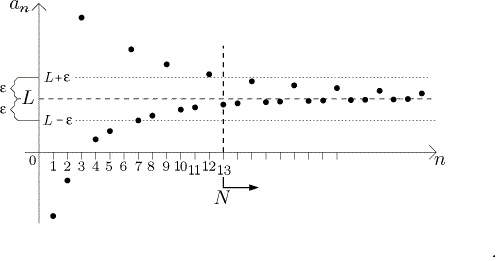
\includegraphics[width=0.45\textwidth]{figures/limit}
\end{figure}

\paragraph{•}
Think of this as a game. If I give you some L that I claim to be the limit of a sequence and you give me some $\epsilon$, no madder how small, can I find some $N$ such that every element in the sequence of index greater than $N$ is within  $L-\epsilon<a_n<L+\epsilon$? If the answer is yes, then the limit of the sequence as $n \to \infty$ is $L$. Put another way, the sequence converges to $L$. Although this may seem intuitive, we must have a formal definition of the convergence of sequences in order to be able work with them.
\subsection*{The Geometric Series}
\paragraph{•}
Lets take a look at the Sequence $S_n = r^n $ where $r$ is a real number. 
\[
\lim_{n\to\infty}r^n = \left\{ 
  \begin{array}{l l}
    0 & \quad \text{if} \quad|r|<1\\
    \infty & \quad \text{if} \quad r>1\\
    -\infty & \quad \text{if} \quad r<1\\
    1 & \quad \text{if} \quad r=1
  \end{array} \right.
  \]
  Keep this in mind as we move on to the Geometric Series
\paragraph{•}
The Geometric Series is defined as $$S_n = \sum_{n = 0}^{n-1}ar^n = a + ar+ ar^2+ar^3+...+ar^{n-2}+ar^{n-1}$$.

Multiplying $S_n$ by $r$ .
\[
rS_n = ar + ar^2 +ar^3+...+ar^{n-1}+ar^n
\]
Subtracting these two sequences .
\[
S_n - rS_n = a + ar+ ar^2+ar^3+...+ar^{n-2}+ar^{n-1}
			-(ar + ar^2 +ar^3+...+ar^{n-1}+ar^n).
\]
Grouping terms.
\[
S_n - rS_n = (a-ar)+ (ar-ar^2)+ (ar^2- ar^3) +...+(ar^{n-2}-ar^{n-1})+(ar^{n-1}-ar^n)
\]
\[
S_n - rS_n = a - ar^n
\]
Solving for $S_n$.
\[
S_n = \frac{a - ar^n}{1-r}
\]
Now we can take the infinite sum of this sequence. 
\[
\sum_{n = 0}^\infty ar^n = \lim_{n\to\infty} \sum_{n = 0}^{n-1} ar^n = \lim_{n\to\infty} a\frac{1-r^n}{1-r} = \frac{a}{1-r} \quad \text{if} \quad |r|<1
\]
\subsection*{The Ratio Test}
Assume that 
\[
\lim_{n\to \infty}\left\lvert{\frac{a_{n+1}}{a_n}}\right\lvert = L<1.
\]
This means that there exists some $N$ such that for all $n>N$ 
\[
L-\epsilon<\frac{a_{n+1}}{a_n}<L+\epsilon \quad \text{ or } \quad  \left\lvert \frac{a_{n+1}}{a_n} -L \right\lvert <\epsilon.
\]
We can choose some $r$ such that $L<r<1$. So for all $n>N$
\[
\left\lvert \frac{a_{N+1}}{a_N}  \right\lvert <r.
\] 
Multiplying both sides of the inequality by $|a_N|$ we get 
\[
|a_{N+1}|<|a_N|r.
\]
Incrementing N,
\[
|a_{N+2}|<|a_{N+1}|r
\] 
and since $r<1$.
\[
|a_{N+1}|r<|a_N|r^2.
\]
So
\[
|a_{N+2}|<|a_N|r^2.
\]
Continuing this pattern we find that 
\[
|a_{N+k}|<|a_N|r^k.
\]
We have not proved the comparison test. However, it should be obvious that 
\[
\sum_{k=1}^\infty |a_{N+k}| < \sum_{k=1}^\infty |a_N|r^k
\]
but we know that 
\[
\sum_{n = 0}^\infty ar^n = \frac{a}{1-r}  \text{ for all } |r|<1
\] 
is the Geometric Series.
\[
\text { So }\sum_{k=1}^\infty |a_N|r^k \text{ will converge when} |r|<1. \text{ We defined r to always be less than 1. So }  \sum_{k=1}^\infty |a_{N+k}| \quad \text{Will also converge.}
\] 
This brings us to one of the most useful test for the convergence of a series: The Ratio test.\newline
\paragraph{•}

\[
\text{Suppose we are given a series defined as }\sum_{k=n}^\infty a_k
\]
if 
\[
\lim_{n\to\infty} \left\lvert \frac{a_{n+1}}{a_n} \right\rvert= L < 1, \text{ then } \sum_{n=1}^\infty a_n \text{ will converge. }
\]
if 
\[
\lim_{n\to\infty} \left\lvert \frac{a_{n+1}}{a_n} \right\rvert = L> 1 \text{, then } \sum_{n=1}^\infty a_n \text{ will diverge. }
\]
if 
\[
\lim_{n\to\infty} \left\lvert \frac{a_{n+1}}{a_n} \right\rvert =  1 \text{, then the test fails, since } \frac{a}{1-r} \text{ results in a divide by 0 error when } r = 1. 
\]
\subsection*{Geometric Series Function Identities}
\paragraph{•}
We know that 
\[
\sum_{n = 0}^\infty ax^n = \frac{a}{1-x}  \text{ for all } |x|<1.
\]
\[
\text{Let's see what happens when we take } \int\sum_{n = 0}^\infty x^n dx
\]
\begin{align*}
\int\sum_{n = 0}^\infty ax^n  &= \int(1+x+x^2+...+x^{n-1}+x^n+...)dx\\
&=x+\frac{x^2}{2}+\frac{x^3}{3}+...+\frac{x^n}{n}+\frac{x^{n+1}}{n+1}+...+c
\end{align*}
so 
\[
\int\sum_{n = 0}^\infty ax^n = \sum_{n=0}^\infty \frac{x^{n+1}}{n+1} + c 
\]
But  $$\int \frac{1}{1-x}dx = -\ln(1-x)+c$$.
So
\[
\sum_{n=0}^\infty \frac{x^{n+1}}{n+1} = -\ln(1-x) + c \text{ for all } |x|<1
\]
Plugging in $x=0$, we get 
\[
0 = -\ln(1) + c
\]
so $c=0$. So 
\[
\ln(1-x) = -\sum_{n=1}^\infty \frac{x^{n}}{n} \text{ for all } |x|<1
\]
\newline
\newline

Now, let's take a look at 
\[
\sum_{n=0}^\infty (-x^2)^n = \frac{1}{1+x^2} \text{ for all } |x|<1 
\]
\begin{align*}
\int\sum_{n=0}^\infty (-x^2)^ndx &= \int(1-x^2+x^4-x^6+...)dx\\
&= x-\frac{x^3}{3}+\frac{x^5}{5}-\frac{x^7}{7}+...+c 
\end{align*}
So 
\[
\int\sum_{n=0}^\infty (-x^2)^ndx = \sum_{n=0}^\infty \frac{(-1)^nx^{2n+1}}{2n+1} + c.
\]
But
\[
\int \frac{1}{1+x^2}dx = \arctan(x) + c
\]
So
\[
\sum_{n=0}^\infty \frac{(-1)^nx^{2n+1}}{2n+1} = \arctan(x) + c \text{ for all } |x|<1
\]
Plugging in $x=0$, we get $c=0$. So 
\[
\arctan(x)=\sum_{n=0}^\infty \frac{(-1)^nx^{2n+1}}{2n+1}  \text{ for all } |x|<1
\]

\subsection*{The Power Series}
\[
\text{The Power Series is defined as } \sum_{n=0}^\infty c_nx^n \text{ where } c_n \text{ is a series of constants called the \textit{coefficient} of the power series.}
\]
so
\[
f(x) = \sum_{n=0}^\infty c_nx^n= c_0+c_1x+c_2x^2+...+c_nx^n.
\]
A power Series centered at $a$ is defined as 
\[
f(x)=\sum_{n=0}^\infty c_n(x-a)^n= c_0+c_1(x-a)+c_2(x-a)^2+...+c_n(x-a)^n.
\]
The \textit{radius of convergence} of a power series is some number $R$ for which the series will converge for all $|x-a|<R$. We can test for the radius of convergence by applying the Ratio Test. For example. 
\paragraph{Example}
\paragraph{•}
Let's take a look at the power series
\[
\sum_{n=1}^\infty \frac{(x+1)^n}{n2^n}
\]
Applying the ratio test.
\[
\lim_{n\to\infty}\left\lvert\frac{(x+1)^{n+1}}{(N+1)2^{N+1}}\times \frac{n2^n}{(x+1)^n}\right\rvert <1
\]
\[
\lim_{n\to\infty}\left\lvert \frac{(x+1)n}{{n+1}}\right\rvert <1
\]
\[
|x+1|\lim_{n\to\infty}\left\lvert \frac{n}{n+1} \right\lvert <1
\]
\[
|x+1|<1
\]
So the radius of convergence of this power series is 1. The interval of convergence is $-3<x<1$.
\paragraph{The Additive Property}
\paragraph{•}
One very important property of the power series is the additive property. Suppose we have two power series, $f(x)$ and $g(x)$, where 
\[
f(x)=\sum_{n=0}^\infty a_n(x-a)^n= a_0+a_1(x-a)+a_2(x-a)^2+...
\]
and
\[
g(x) = \sum_{n=0}^\infty b_n(x-a)^n= b_0+b_1(x-a)+b_2(x-a)^2+....
\]
\begin{align*}
f(x)\pm g(x) &= (a_0+a_1(x-a)+a_2(x-a)^2+...) \pm (b_0+b_1(x-a)+b_2(x-a)^2+...).\\
&= (a_0 \pm b_0)+(a_1 \pm b_1)(x-a)+(a_2 \pm b_2)(x-a)^2 +...
\end{align*}
So 
\[
f(x)\pm g(x) = \sum_{n=1}^\infty (a_n \pm b_n)(x-a)^n
\]
\paragraph{Differentiating and Integrating a Power Series}
\paragraph{•}
Now, let's take a look at $\dfrac{d}{dx} f(x)$.
\begin{align*}
\dfrac{d}{dx} f(x) &= \frac{d}{dx} \sum_{n=0}^\infty a_n(x-a)^n\\
& = \frac{d}{dx}[a_0+a_1(x-a)+a_2(x-a)^2+...]\\
& = a_1 + 2a_2(x-1)+ 3a_3(x-a)^2+...
\end{align*}
so 
\[
\frac{d}{dx} \sum_{n=0}^\infty a_n(x-a)^n = \sum_{n=1}^\infty na_n(x-a)^{n-1}
\]
Similarly 
\[
\int \sum_{n=0}^\infty a_n(x-a)^n = \sum_{n=0}^\infty \frac{a_n(x-a)^{n+1}}{n+1} + c
\]
\subsection*{Maclaurin Series and Taylor Series}

\paragraph{The Maclaurin Series}
\paragraph{•}
The idea behind the Maclaurin Series is that if we have some function, we can approximate that function about a certain interval by building a polynomial whose derivatives match those the function's at 0. In other words, if we have some function $f$ that is differentiable at $0$ we can call our approximation $P$. So
\begin{align*}
&P(0) = f(0)\\
&P'(0) = f'(0)\\
&P''(0) = f''(0)\\
&...\\
&P^{(n)}(0) = f^{(n)}(0)
\end{align*}
and we can build a polynomial that looks like
\[
p(x) \approx f(0) + f'(0)x + \frac{f''(0)}{2}x^2 + \frac{f'''(0)}{6}x^3 +....+ \dfrac{f^{(n)}(0)}{n!}x^n
\]
So we get something that looks like this.
\begin{figure}[H]
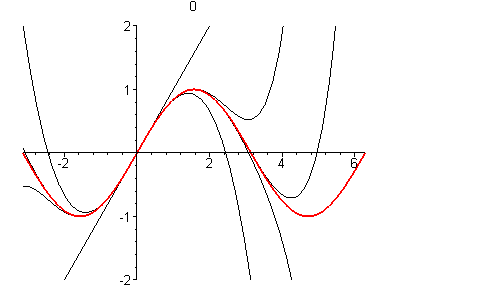
\includegraphics[width=0.45\textwidth]{figures/Taylor1}
\caption{Maclaurin Series approximation of $\sin(x)$}
\end{figure}

\paragraph{The Taylor Series}
\paragraph{•}
The Taylor Series simply takes this idea and expands it work for points other than $0$.
If we have some function $f(x)$ we can shift that function to the right $a$ places by passing the argument $x-a$. So we can take the Maclaurin Series and apply it to any point $a$ by creating the polynomial
\[
p(x) \approx f(a) + f'(a)(x-a) + \frac{f''(a)}{2}(x-a)^2 + \frac{f'''(a)}{6}(x-a)^3 +....+ \dfrac{f^{(n)}(a)}{n!}(x-a)^n
\]
So we get something that looks like this.
\begin{figure}[H]
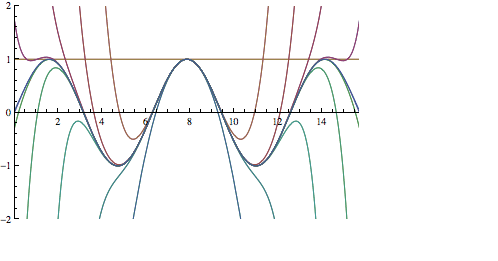
\includegraphics[width=0.45\textwidth]{figures/Taylor2}
\caption{Taylor Series approximation of $\sin(x)$. In this case, $a=\frac{5\pi}{2}$}
\end{figure}
This is known as the Taylor Series.
\paragraph{•}
We can test the radius of convergence of a Taylor series by applying to ratio test.
For example take the Taylor series expansion of $e^x$ centered at 0.
\[
e^x \approx 1 + x + \frac{x^2}{2} + \frac{x^3}{3!} +\frac{x^4}{4!}+....+\frac{x^n}{n!}
\]
so 
\[
e^x \approx \sum_{n=0}^N \frac{x^n}{n!}
\]
Applying the ratio test.
\[
\lim_{n\to\infty} \left\lvert \frac{x^{n+1}}{(n+1)!} \times \frac{n!}{x^n}\right\rvert
=x\lim_{n\to\infty} \left\lvert \frac{1}{n+1} \right\rvert 
= 0
\]
and $0<1$ for all $x$. So
\[
e^x = \sum_{n=0}^\infty \frac{x^n}{n!} \text{ for all  }x.
\]
We can use the same method for $\sin(x)$ and $\cos(x)$.
\[
\cos(x) \approx 1 - \frac{x^2}{2} + \frac{x^4}{4!} - \frac{x^8}{8!} + \frac{x^{10}}{10!} +.....+\frac{(-1)^{n}x^{2n}}{2n!}
\]
\[
\sin(x) \approx x - \frac{x^3}{3!} + \frac{x^5}{5!} - \frac{x^7}{7!} + \frac{x^9}{9!} +....+ \frac{(-1)^nx^{2n+1}}{(2n+1)!}
\]
Applying the ratio test to both of these Taylor Series expansions we can come to the conclusion that 
\[
\cos(x) = \sum_{n=0}^\infty \frac{(-1)^{n}x^{2n}}{2n!} \text{ for all }x
\]
and
\[
\sin(x) = \sum_{n=0}^\infty \frac{(-1)^nx^{2n+1}}{(2n+1)!} \text{ for all }x.
\]

\section{Series Approximation of Differential Equations}
\paragraph{•}
Let's get back to the real subject at hand. Differential Equations! We have learned of  some very special cases of differential equations that can be solved analytically. However, not all, in fact most differential equations can not be solved by such means. We can use what we know about series to find a Power Series representation of solutions to many homogeneous differential equations in the form of 
\[
P(x)y''+Q(x)y'+R(x)y = 0.
\] 
\paragraph{•}
A differential equation is said to be analytic if both 
\[
\frac{Q(x)}{P(x)} \quad \textbf{and} \quad \frac{R(x)}{P(x)}
\]
have a Taylor Series representation about the \textit{ordinary} point $x=x_0$. A point that is not ordinary is called a \textit{singular point}. If $x=x_0$ were a singular point, this would mean that $P(x_0) = 0$. For example, the equation 
\[
y''(x-1)+y = 0
\]
would have a singular point at $x=1$. We will get to singular points later. For now, we can content ourselves with differential equations that have no singular points.
\subsection*{Example}
\paragraph{}
The first method we will cover can be best represented by an example.

\[
\textit{Determine a series solution to the following differential equation about the point }x=x_0 	
\]
\[
y''+y = 0
\]
The first thing we do is assume that 
\[
y=\sum_{n=0}^\infty a_nx^n \text{,}\quad y'= \sum_{n=1}^\infty na_nx^{n-1} \quad \text{, and} \quad y''= \sum_{n=2}^\infty n(n-1)x^{n-2}
\]
so
\[
\sum_{n=2}^\infty n(n-1)x^{n-2} + \sum_{n=0}^\infty a_nx^n = 0
\]
We can shift the power series for $y''$ so that both series have the same exponent.
\[
\sum_{n=0}^\infty a_{n+2}(n+2)(n+1)x^n + \sum_{n=0}^\infty a_nx^n = 0
\]
Using the additive identity.
\[
\sum_{n=0}^\infty [a_{n+2}(n+2)(n+1) + a_n]x^n = 0
\]
Because this power series is zero for all $x$, all of the coefficients of the power series must be equal to zero. So 
\[
a_{n+2}(n+2)(n+1) + a_n = 0
\]
\[
a_{n+2} = - \frac{a_n}{(n+2)(n+1)}
\] 
This is referred to as a \textit{recurrence relation}. We can now iterate though the values of $n$ in the hopes of finding a \textit{closed form} of $a_n$.
\begin{align*}
&n=0: \ &n=1:\ 
\\ &a_2 = - \frac{a_0}{2\cdot1}  \ &a_3 = -\frac{a_1}{2\cdot3} \ 
\\ \\
&n= 2: \ &n=3: \
\\&a_4 = -\frac{a_2}{4\cdot3} = \frac{a_0}{4\cdot3\cdot2\cdot1} \ &a_5 = -\frac{a_3}{5\cdot4} = \frac{a_1}{5\cdot4\cdot3\cdot2\cdot1} \
\\ \\
&n=4: \  &n=5 \
\\
a_6 &= -\frac{a_4}{6\cdot5} = -\frac{a_0}{6\cdot5\cdot4\cdot3\cdot2\cdot1}
\ &a_7=-\frac{a_5}{7\cdot6}=-\frac{a_1}{7\cdot6\cdot5\cdot4\cdot3\cdot2\cdot1} \
\end{align*}
\paragraph{•}
It would seem as though all of the even values of $n$ involve an $a_0$ and the odd powers involve an $a_1$. This leads us to believe that there are two solutions to the differential equation, which makes sense since it is a second order differential equation. So now we let $n = 2k$. So
\[
a_{2k} = \frac{(-1)^k}{2k!}a_0 \quad \text{and} \quad a_{2k+1} = \frac{(-1)^k}{(2k+1)!}a_1.
\]
Now all we need to do is write out the first few terms of our solution in order to see our final result.
\begin{align*}
y&=\sum_{n=0}^\infty a_nx^n 
\\
&= a_0+a_1x+a_2x^2+a_3x^3+...+a_nx^n+...
\\
&= a_0 +a_1x-\frac{a_0}{2!}x^2-\frac{a_1}{3!}x^3+...+\frac{(-1)^n}{2k!}a_0+\frac{(-1)^n}{(2k+1)!}a_1+...
\\
&= a_0\sum_{n=0}^\infty\frac{(-1)^n}{2k!}x^{2n} + a_1\sum_{n=0}^\infty \frac{(-1)^n}{(2k+1)!}x^{2n+1}
\\
&= a_0\cos(x) + a_1\sin(x) \quad \text{for all }x 
\end{align*}
\section{Euler Equations About an Ordinary Point}
\subsection*{ The Euler Equation}
\paragraph{•}
The \textit{Euler Equation} can be defined as 
\[
L[y] = x^2y''+\alpha xy'+\beta y = 0. \text{ Where } \alpha \text{ and } \beta \text{ are constants.}
\] 
Since $P(x) = x^2$, $x=0$ is the only singular point. First, let's take a look at the case where $x>0$.
\[
\text{Assume that }y=x^r \text{ is a solution.}
\]
\[
\frac{d}{dx}x^r = rx^{r-1}, \quad \frac{d^2}{dx^2}x^r = r(r-1)x^{r-2}.
\]
\[
L[x^r]= x^2\frac{r^2}{x^2}r(r-1) + \alpha x\frac{x^r }{x}r+\beta x^r = 0
\]
\[
x^r[r(r-1)+\alpha r + \beta] = 0
\]
\[
\text{So } x^r = 0 \quad \text{and} \quad r(r-1)+\alpha r + \beta= 0
\]
Now we can solve this second equation for $r$.
\begin{align*}
F(r) &= r(r-1)+\alpha r + \beta= 0 \\
&= r^2-r+\alpha r+ \beta = 0 \\
&= r^2 +r(\alpha - r)+ \beta = 0\\
r_1,r_2 &= \frac{-(\alpha - 1) \pm \sqrt{(\alpha - 1)^2-4\beta}}{2}
\end{align*}
So 
\[
y_1(x) = x^{r_1}, \quad \text{ and } \quad y_2(x)= x^{r_2}.
\]
Taking the Wronskain 
\[
W[r_1,r_2] = (r_2-r_1)x^{r_1+r_2-1} \neq 0 
\]
\[
\text{So given a differential equation in the form of }  x^2y''+\alpha xy'+\beta y = 0, 
\]
\[
y = c_1x^{r_1}+c_2x^{r_2} \quad \forall (r_1 \neq r_2) \in \mathbb R, x>0
\]

\subsection{Repeated roots}
\paragraph{•}
Now, let's see what happens when $r_1 = r_2$. First, recall that if we have some polynomial $P(x)$ which has roots at $x_0$, that is to say $P(x_0) = 0$, of multiplicity $n$, then $P(x) = p(x)(x-x_0)^n$ where $p(x)$ is another polynomial that does not have roots at $x_0$. So in the case of the function 
\[
 F(r) = r(r-1)+\alpha r + \beta= 0,
\]
if $r_1 = r_2$, then $F(r)$ has roots at $r = r_1$ of multiplicity $2$. So 
\[
 F(r) = (r-r_1)^2. 
\]
So now we differentiate $L[x^r]$ with respect to $r$.
\[
\frac{\partial}{\partial r}L[x^r] = \frac{\partial}{\partial r}[x^rF(r)] = \frac{\partial}{\partial r}[x^r(r-r_1)^2] = x^r \ln(x)(r-r_1)^2 + 2r(r-r_1) = 0\quad
\text{ for all }r=r_1.
\]
\[
\text{But } \frac{\partial}{\partial r}L[x^r] = L\left[\frac{\partial}{\partial r}x^r\right] = L[x^r \ln(x)]  
\]

\[
\text{But since we know that } \frac{\partial}{\partial r}L[x^r] = 0, \quad  L[x^r \ln(x)]  = 0
\] 
\[
\text{So } y_2 = x^{r_1}\ln(x), x>0
\]
\[
\text{So } y = x^{r_1}[c_1 + c_2 \ln (x)]
\]
\subsection{Complex Roots}
\paragraph{•}
Now let's see what happens when $r_1,r_2 = \lambda \pm \mu i $.
\[
x^r = e^{r \ln (x)}
\]
\[
x^{ \lambda + \mu i} = e^{( \lambda + \mu i)\ln (x)} = e^{\lambda \ln (x)}e^{\mu i \ln (x)} = x^\lambda e^{\mu i \ln (x)}
\]
\[
= x^\lambda[\cos(\mu \ln x) + i \sin(\mu \ln x)]\quad  x> 0 
\]
\[
\text{So } y = x^\lambda[c_1\cos(\mu \ln x)+ c_2 \sin (\mu \ln x)]\quad x> 0 
\]
\subsection{x Less Than Zero}
\paragraph{•}
So, what happens if $x<0$? Let's take a look at the differential equation in the form of 
\[
L[y] = x^2y''+\alpha xy'+\beta y = 0. \text{ Where } \alpha \text{ and } \beta \text{ are constants and }x<0 
\]
We can let 
\[
  x = -\nu \quad \text{and} \quad y = \zeta(\nu).
\] 
So 
\[
y'=\frac{d \zeta}{d \nu}\frac{d\nu}{dx} = -\frac{d \zeta}{d\nu}, \quad \text{and} \quad y''= \frac{d}{d \nu}\left[-\frac{d \zeta}{d \nu}\right]\left( \frac{d \nu}{dx}  \right) = \frac{d^2\zeta}{d\nu^2}
\]
Plugging these identities back into the Euler Equation, We get 
\[
L[\zeta] = x^2\zeta '' + \alpha x \zeta ' + \beta \zeta
\] 
And so all of the work that we just did regarding the Euler Equation will apply to all $x\neq 0$! 
\subsection{Bringing it All Together}
\paragraph{•}
Let's recap. A differential equation in the form of 
\[
L[y] = x^2y''+\alpha xy'+\beta y = 0. \text{ Where } \alpha \text{ and } \beta \text{ are constants.}
\]
Can be reduced to the characteristic equation 
\[
 F(r) = r(r-1)+\alpha r + \beta= 0,
\]

 $\bullet \text{ If }  r_1,r_2 \in \mathbb{R} \text{ and }r_1 \neq r_2 $
 
 \[
 r_1,r_2 = \frac{-(\alpha - 1) \pm \sqrt{(\alpha - 2)^2 - 4\beta}}{2} \quad \text{and} \quad y = c_1|x|^{r_1}+c_2|x|^{r_2} \quad x \neq  0
 \]
$\bullet \text{ If } r_1,r_2 \in \mathbb{R} \text{ and }r_1 = r_2 $
 
 \[
 y = |x|^r(c_1+c_2 \ln |x| )  \quad x \neq  0
 \] 
 
 $\bullet \text{ If } r_1,r_2 = \lambda \pm \mu i$
 
 \[
 y = |x|^\lambda[c_1 \cos ( \mu \ln |x|)+ c_2 \sin( \mu \ln |x| )] \quad  x \neq  0
 \]
 
  
  \section{Series Approximation near a Singular Point}
  \subsection{Regular vs. Irregular Singular points}
 \paragraph{•}
 Say we are given a differential equation in the form of 
 \[
 P(x)y'' + Q(x)y' + R(x) y = 0
 \]
 and $P(x)$ has a root point at $x_0$ of multiplicity $n$, $Q(x)$ has a root at $x_0$ of multiplicity $m$, and $R(x)$ has a root at $x_0$ of multiplicity $k$.
  We can say that 
  \begin{align*}
  &P(x) = p(x)(x-x_0)^n \quad \text {where } p(x_0) \neq 0, \\
  &Q(x) = q(x)(x-x_0)^m \quad \text {where } q(x_0) \neq 0, \text{ and } \\
  & R(x) = r(x) (x-x_0)^k \quad \text  {where } r(x_0) \neq 0.
  \end{align*}

  So, if we were to divide the given differential equation by $P(x)$, then 
  \begin{align*}
  \frac{Q(x)}{P(x)} = \frac{p(x)(x-x_0)^m}{q(x)(x-x_0)^n} \quad \text{and}  \quad
  \frac{R(x)}{P(x)} = \frac{r(x)(x-x_0)^k}{q(x)(x-x_0)^n}. 
  \end{align*}
  So, if $n>m$ or $n>k$, then we will have a divide by zero error at $x_0$. However, if $m \geq n $ and $k \geq n$, we will no longer have this problem. A singular point is considered regular if $m+1 \geq n$ and $k+2 \geq n$. In other words, if 
  \[
  \lim_{x \to x_0} (x-x_0)\frac{Q(x)}{P(x)} \quad \text{is finite, and} 
  \]
  \[\lim_{x \to x_0} (x-x_0)^2 \frac{R(x)}{P(x)} \quad \text{is finite.}
  \]
  Then $x_0$ is a regular singular point. Although this may not seem very useful at the moment, we will soon see that a regular singular point is much easier to work with than an irregular one.
  \subsection{Series Approximation Near a Regular Singular Point}
  Lets assume that our differential equation 
  \[
  P(x)y'' + Q(x)y' + R(x) y = 0
  \]
  has a regular singular point at $x = 0$. We can divide this equation by $P(x)$ and multiply it by $x^2$ to get 
  \[
  x^2y''+x[xp(x)]y'+x^2q(x)y = 0 
  \]
  \[\quad \text{where} \quad p(x) =  \frac{Q(x)}{P(x)} \text{ and } q(x) =   \frac{R(x)}{P(x)}.
  \]
  Since we have assumed that $x= 0$ is a regular singular point, 
 \[
 \lim_{x \to 0} xp(x) \quad \text{and} \quad \lim_{x \to 0} x^2q(x) \quad \text{ are finite.}
 \]
 So they will also have a convergent power series approximation near $x=0$. So let's say that 
 \begin{align*}
 &xp(x) = \sum_{n=0}^\infty p_n x^n \quad \\
 \text{and }\\
 &x^2q(x) = \sum_{n=0}^\infty q_n x^n. 
 \end{align*}
 so 
 \begin{align*}
 &\lim_{x \to 0}xp(x) = \lim_{x \to 0} (p_0 +p_1x+p_2x^2+...) = p_0  \\
 \text{and }\\
 &\lim_{x \to 0}x^2q(x) = \lim_{x \to 0} (q_0 +q_1x+q_2x^2+...) = q_0
\end{align*} 
So the given differential equation can be reduced to 
\[
x^2y''+xp_0y'+q_0y = 0  
\]
near the point $x=0$.  But this is the Euler equation that was discussed in previous sections, which has the solution $x^r$. So we can assume that 
\[
y = x^r \sum_{n=0}^\infty a_nx^n = \sum_{n=0}^\infty x^{n+r}
\]
\section*{Example}
\[
\textit{Find the series approximation near the singular point of the following differential equation.}
\]
\[
2xy''+y'+xy = 0
\]
First we need to find the \textit{indicial equation}.
\[
p_0 = \lim_{x \to 0}x\frac{1}{2x} = \frac{1}{2} \quad q_0 = \lim_{x \to 0} x^2\frac{x}{2x} = 0
\]
so 
\[
x^2y'' +\frac{1}{2}xy' = 0
\]
\[
r(r-1)+\frac{1}{2}r= 0
\]
This is known as the\textit{indicial equation}. Solving for $r$. 
\[
r=0 \quad,\quad r = \frac{1}{2}
\]
So we assume that 
\[
y = \sum_{n=0}^\infty a_nx^{n+r}\quad,\quad y' = \sum_{n=0}^\infty (n+r)a_nx^{n+r-1} \quad \text{, and } \quad y'' = \sum_{n=0}^\infty (n+r)(n+r-1)a_nx^{n+r-2}
\]
so 
\[
2\sum_{n=0}^\infty (n+r)(n+r-1)a_nx^{n+r-1} + \sum_{n=0}^\infty (n+r)a_nx^{n+r-1} + \sum_{n=0}^\infty a_nx^{n+r+1} = 0
\]
shifting the indices.
\[
2\sum_{n=0}^\infty (n+r)(n+r-1)a_nx^{n+r-1} + \sum_{n=0}^\infty (n+r)a_nx^{n+r-1} + \sum_{n=2}^\infty a_{n-2}x^{n+r-1} = 0
\] 
\[
2r(r-1)a_0x^{r-1} + 2(1+r)ra_1x^{n+r}+ra_0x^{r-1}+(1+r)a_1x^{n+r} = 0
\]
\[
a_0[2r(r-1)+r] = 0
\]
Notice that this the \textit{indicial equation}. So once again, we have arrived at the conclusion that 
\[
r=0 \quad,\quad r = \frac{1}{2}
\]
also,
\[
a_1[2(1+r)+(1+r)]= 0
\]
so
\[
a_1 = 0
\]
\[
\sum_{n=2}^\infty[2(n+r)(n+r-1)a_n + (n+r)a_n + a_{n-2}]x^{n+r-1}= 0
\]
\[
a_n = -\frac{a_{n-2}}{(n+r)(2n+2r-1)}
\]
Since $a_1=0$, all of the odd terms will be zero.
\begin{align*}
&r=0 \ &r=\frac{1}{2} \ 
\\
&a_n = -\frac{a_{n-2}}{n(2n-1)} \ &a_n = -\frac{a_{n-2}}{n(2n+1)} \
\\
 n=2:
\\
&a_2 = -\frac{a_0}{2\cdot3} \ &a_2 = -\frac{a_0}{2\cdot5} \
\\
n = 4
\\
&-\frac{a_2}{4\cdot7} = \frac{a_0}{2\cdot4\cdot3\cdot7} \ &a_4 = -\frac{a_2}{4\cdot9}=\frac{a_0}{2\cdot4\cdot5\cdot9} \
\\
n=6
\\
&a_6 = -\frac{a_4}{6\cdot11} = -\frac{a_0}{2\cdot4\cdot6\cdot3\cdot7\cdot11} \ &a_6=-\frac{a_4}{6\cdot13} = -\frac{a_0}{2\cdot4\cdot6\cdot5\cdot9\cdot13}\
\\
\text{generally:}
\\
&a_{2k} = \frac{(-1)^ka_0}{(2k)!!\prod_{j=1}^k(4j-1)} \ &a_{2k} = \frac{(-1)^ka_0}{(2k)!!\prod_{j=1}^k(4j+1)} \
\end{align*} 
so 
\[
y = \sum_{k=1}^\infty   \frac{(-1)^ka_0x^{2k}}{(2k)!!\prod_{j=1}^k(4j-1)} + x^{\frac{1}{2}}\sum_{k=1}^\infty  \frac{(-1)^ka_0x^{2k}}{(2k)!!\prod_{j=1}^k(4j+1)}
\]
\end{document}
